\vspace*{5mm}

\begin{enumerate}
	\item {
		\textbf{ \large Approach} \\
		
		To implement a pipeline architecture with a distributed system, we first break the application task into sub tasks. These sub tasks will in fact be major macro tasks of the application and according to number of sub tasks, the workers would be chosen and assigned those tasks. These workers become the stages of the pipeline. 
	}

	\item {
		\textbf{ \large System Architecture} \\
		
		\begin{figure}[!h]
			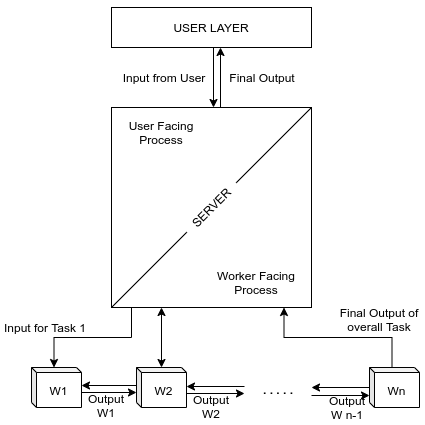
\includegraphics[scale=1]{img/arch.png}
		\end{figure}
	
		\vspace*{3mm}
		
		\pagebreak
		
		The above architecture has two  major components:
		
		\begin{enumerate}
			\item {
				\textbf{Server:} It will be responsible for maintaining the network and controlling the workers along with deploying the application over the network. The server is divided into two logical halves based on what type of process it will handle. It shows the two major processes running on the server:
				
				\begin{enumerate}
					\item {
						\textbf{User Facing Process}: This logical side of the server which will take input from the user to run an application over the pipelined workers. It will provide an interface in the form of a terminal window or a custom graphical user interface to the user to run their application.
					}
				
					\item {
						\textbf{Worker Facing Process}: This side of the server will accept input from the user facing side of the server and will be responsible for dividing up the task into stages for the pipeline. Once it divides the tasks, worker nodes are chosen for the pipeline depending upon the number of stages needed for the application. Each stage is given to a worker node. This side also maintains the status of the workers along with communicating with neighboring workers for input, output or running status update.
					}
					
				\end{enumerate}
			}
		
			\item {
				\textbf{Workers:}
				
				\begin{enumerate}
					\item They will be responsible for computation of the task or the application and return successful output back to the server.
					
					\item The computation will be divided between \textbf{N} workers where the output of one stage will be input for the second and so on.
					
					\item Each stage or worker is dependent upon the output coming from the previous stage
					
					\item The workers in the pipeline will be chosen according to the need of the application. For example, If the application needs 3 interconnected stages in the pipeline, 3 workers would be chosen where the first worker will receive input from the server and the last worker will return the output to the server.
				\end{enumerate}
			}
		\end{enumerate}
	}
\end{enumerate}